\documentclass[11pt,letterpaper]{article}

\usepackage[margin=1in]{geometry}
\usepackage{booktabs}
\usepackage{graphicx}
\usepackage{caption}
\usepackage{amsmath}
\usepackage{hyperref}
\usepackage{parskip}
\usepackage{microtype}
\usepackage{siunitx}

\sisetup{separate-uncertainty=true}

\begin{document}

\noindent{\LARGE\bfseries SHS Lab Test --- 2026-06-29\par}
\vspace{0.4ex}
\noindent{\large Clark South Ballast Tank, WHOI\par}
\vspace{1.0ex}
\noindent Yu Gao; Emerson Hasbrouck; Tom Farrar; Simon de Szoeke; Steven Jayne; Alexander Ekholm\par
\vspace{0.4ex}
\noindent Test date: 2026-06-29. The data record also includes the 2026-06-30 plastic-wick follow-up and post-test data through 2026-07-01 16:18 UTC.\par
\bigskip\hrule\bigskip

\section{Setup}

The test repeated the 2026-05-28 dunk-cycle workflow with two configurations.
On 2026-06-29 the lab test was run in the original wick setup; the fan was raised to
maximum after the first OUT event. The 2026-06-30 follow-up changed to a plastic
friction-fit wick at 12:55 UTC, with the fan turned on at the first IN.

\begin{center}
\begin{tabular}{lll}
\toprule
Instrument & ID & Rate \\
\midrule
RBRduo3 T.T (dry/wet bulb) & SN 233860 & 3 s \\
Vaisala WXT520 (met) & ASWXT203 & 1 min \\
Tank CT reference & --- & 1 Hz nominal \\
\bottomrule
\end{tabular}
\end{center}

\subsection*{Event Log}

\begin{center}
\begin{tabular}{lllr}
\toprule
Cycle & IN & OUT & Duration \\
\midrule
J29-IN-1 & 06-29 15:28 & 15:33 & 5 min \\
J29-IN-2 & 06-29 16:03 & 16:10 & 7 min \\
J29-IN-3 & 06-29 16:37 & 16:40 & 3 min \\
J29-IN-4 & 06-29 17:18 & 17:23 & 5 min \\
J29-IN-5 & 06-29 17:58 & 18:04 & 6 min \\
J29-IN-6 & 06-29 18:40 & 18:44 & 4 min \\
J29-IN-7 & 06-29 19:15 & 19:20 & 5 min \\
J29-IN-8 & 06-29 19:56 & 19:59 & 3 min \\
J30-IN-1 & 06-30 13:08 & 13:14 & 6 min \\
J30-IN-2 & 06-30 13:46 & 13:50 & 4 min \\
J30-IN-3 & 06-30 14:23 & 14:29 & 6 min \\
J30-IN-4 & 06-30 14:58 & 15:30 & 32 min \\
J30-IN-5 & 06-30 16:02 & 16:08 & 6 min \\
\bottomrule
\end{tabular}
\end{center}

\subsection*{Ambient Conditions}

\begin{center}
\begin{tabular}{lrrrr}
\toprule
Phase & T (\si{\degreeCelsius}) & RH (\%) & p (mbar) & wind (m/s) \\
\midrule
2026-06-29 original wick & 21.33 & 72.5 & 1016.82 & 0.94 \\
2026-06-30 plastic wick & 21.21 & 72.9 & 1018.09 & 0.76 \\
\bottomrule
\end{tabular}
\end{center}

\section{Source Notes and Photos}

\subsection*{Testing Notes}
The testing notes are reflected in the setup description and event log above.
They record RBR/WXT startup at 14:50 UTC, fan level 2 at 15:23 UTC, tank CT
logging at 15:27 UTC, the first SHS dunk at 15:28--15:33 UTC, and the fan
increase to maximum after the first OUT event with both probes facing the fan.
For the follow-up, the notes record the 12:55 UTC change to the plastic
friction-fit wick and the five subsequent dunk cycles.

\begin{figure}[p]
  \centering
  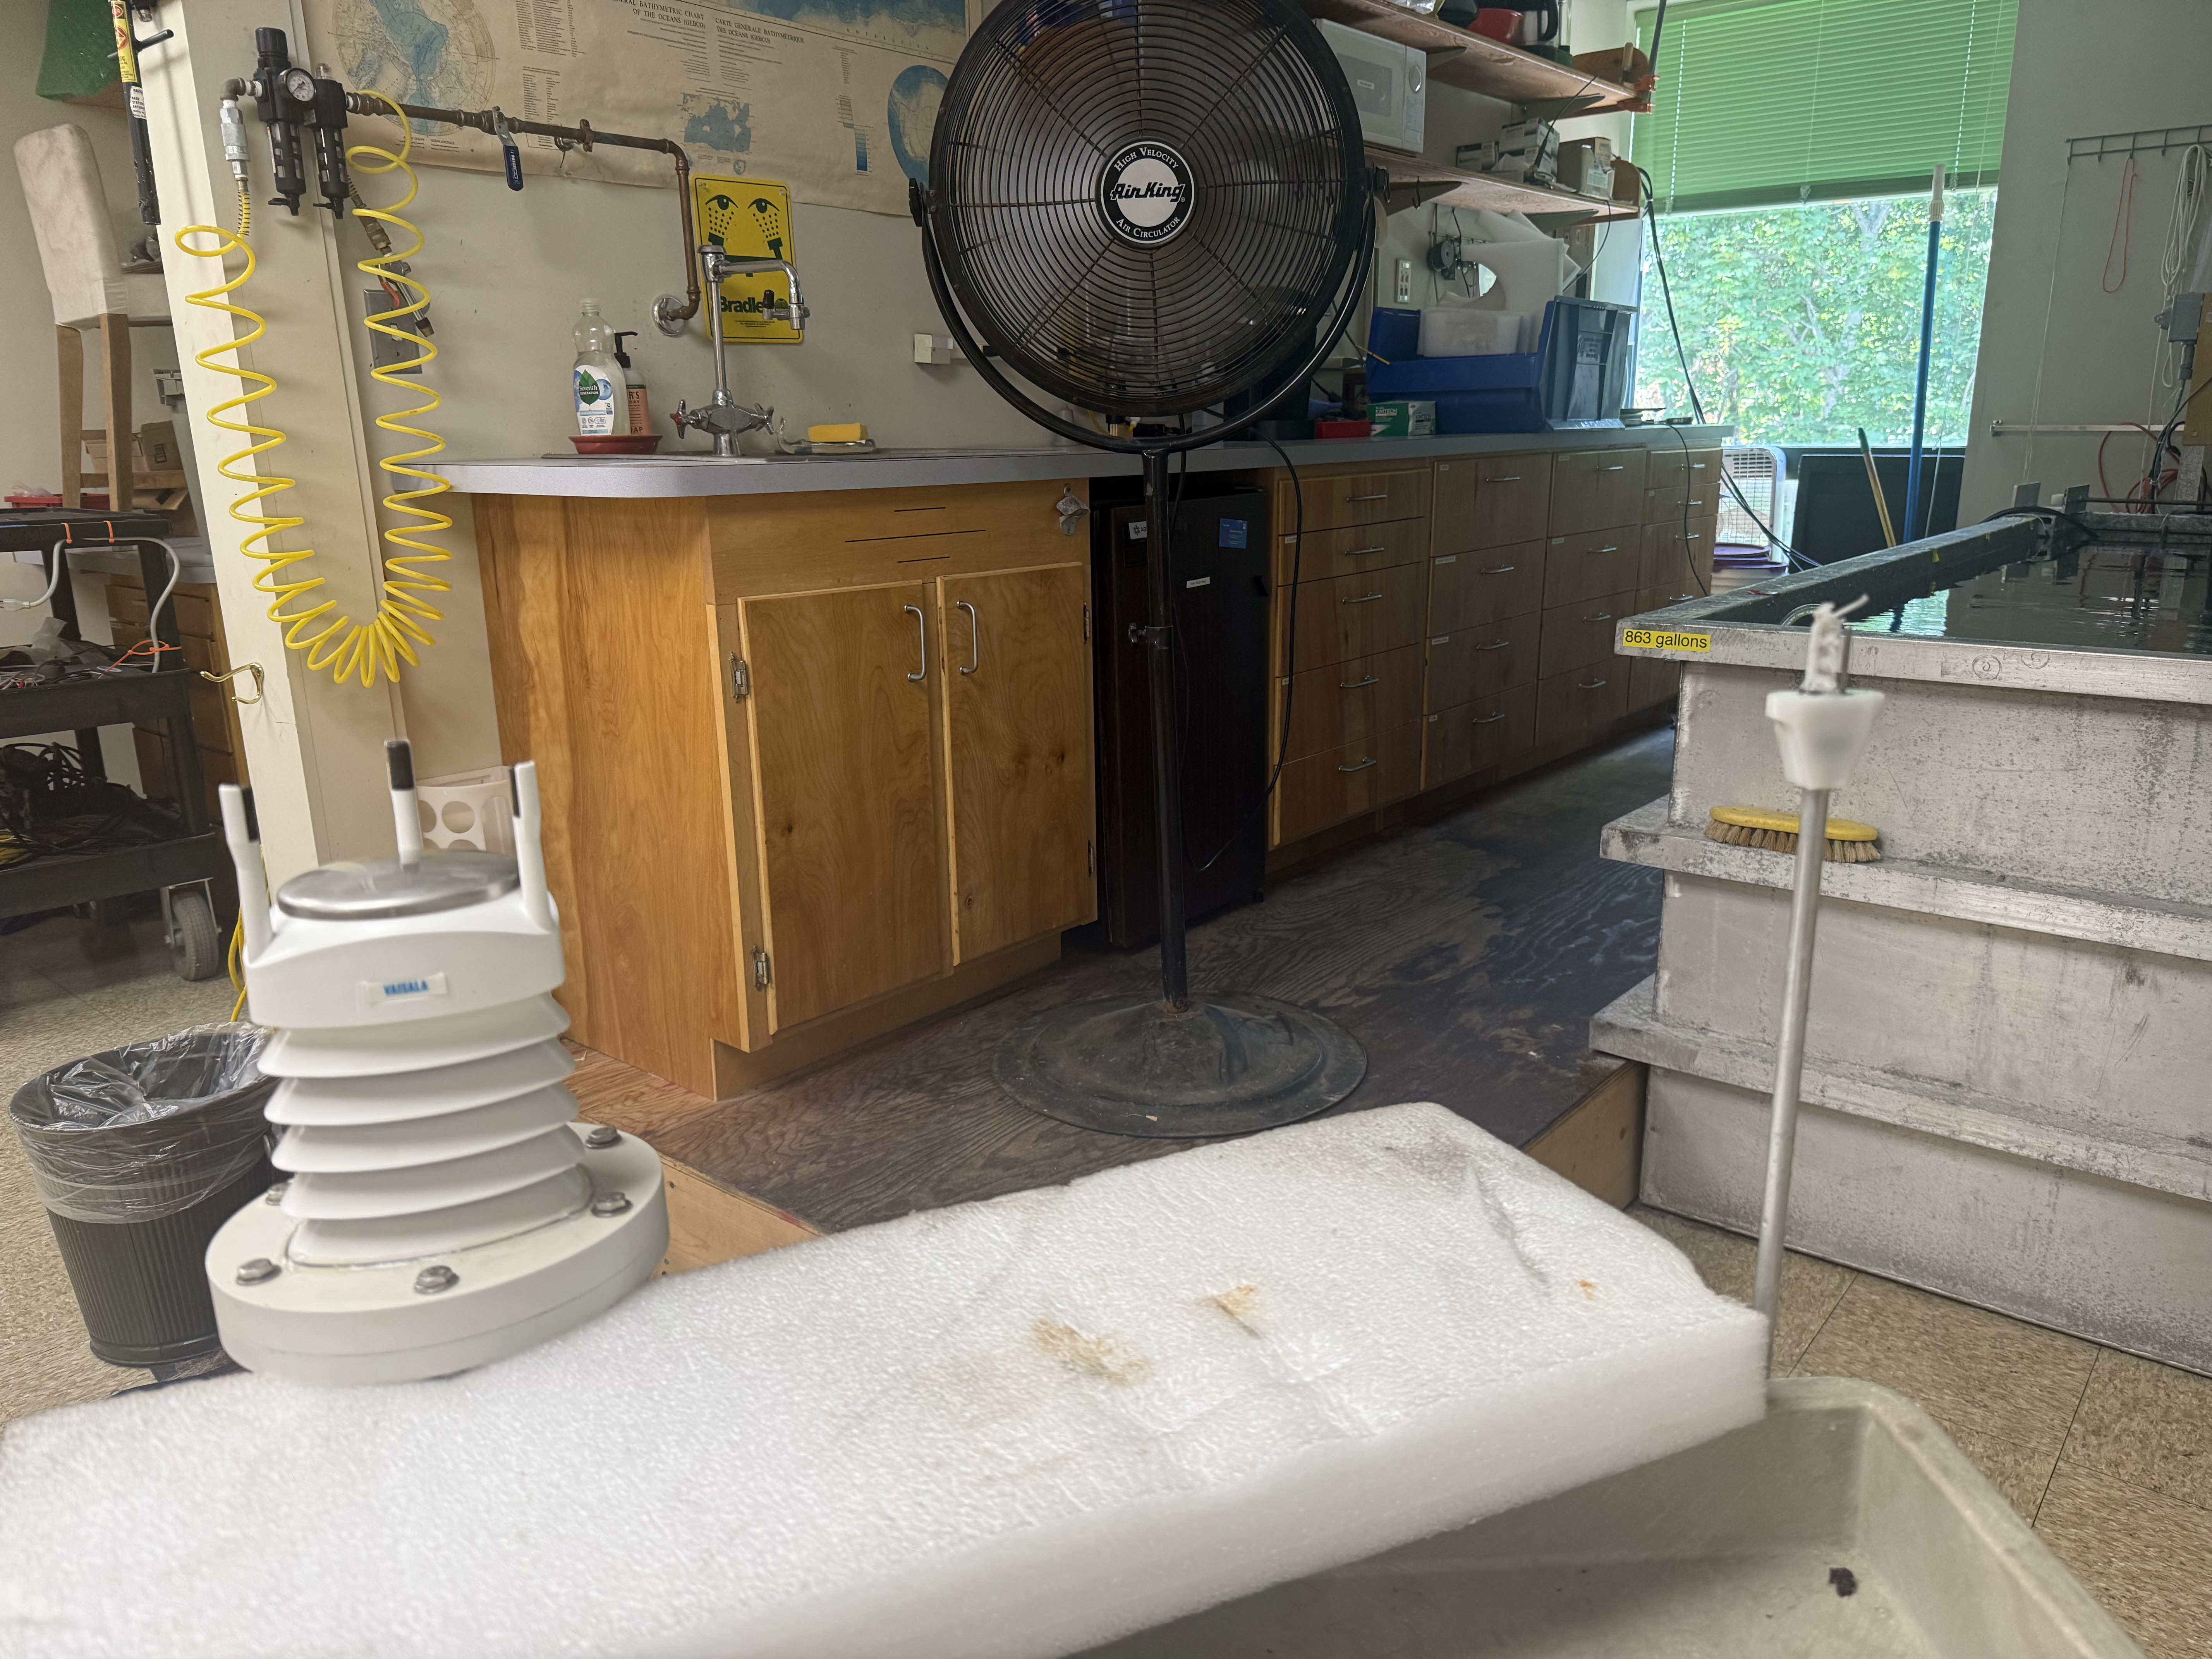
\includegraphics[width=0.48\linewidth,height=0.24\textheight,keepaspectratio]{../../data/20260629Lab/IMG_7609.jpeg}\hfill
  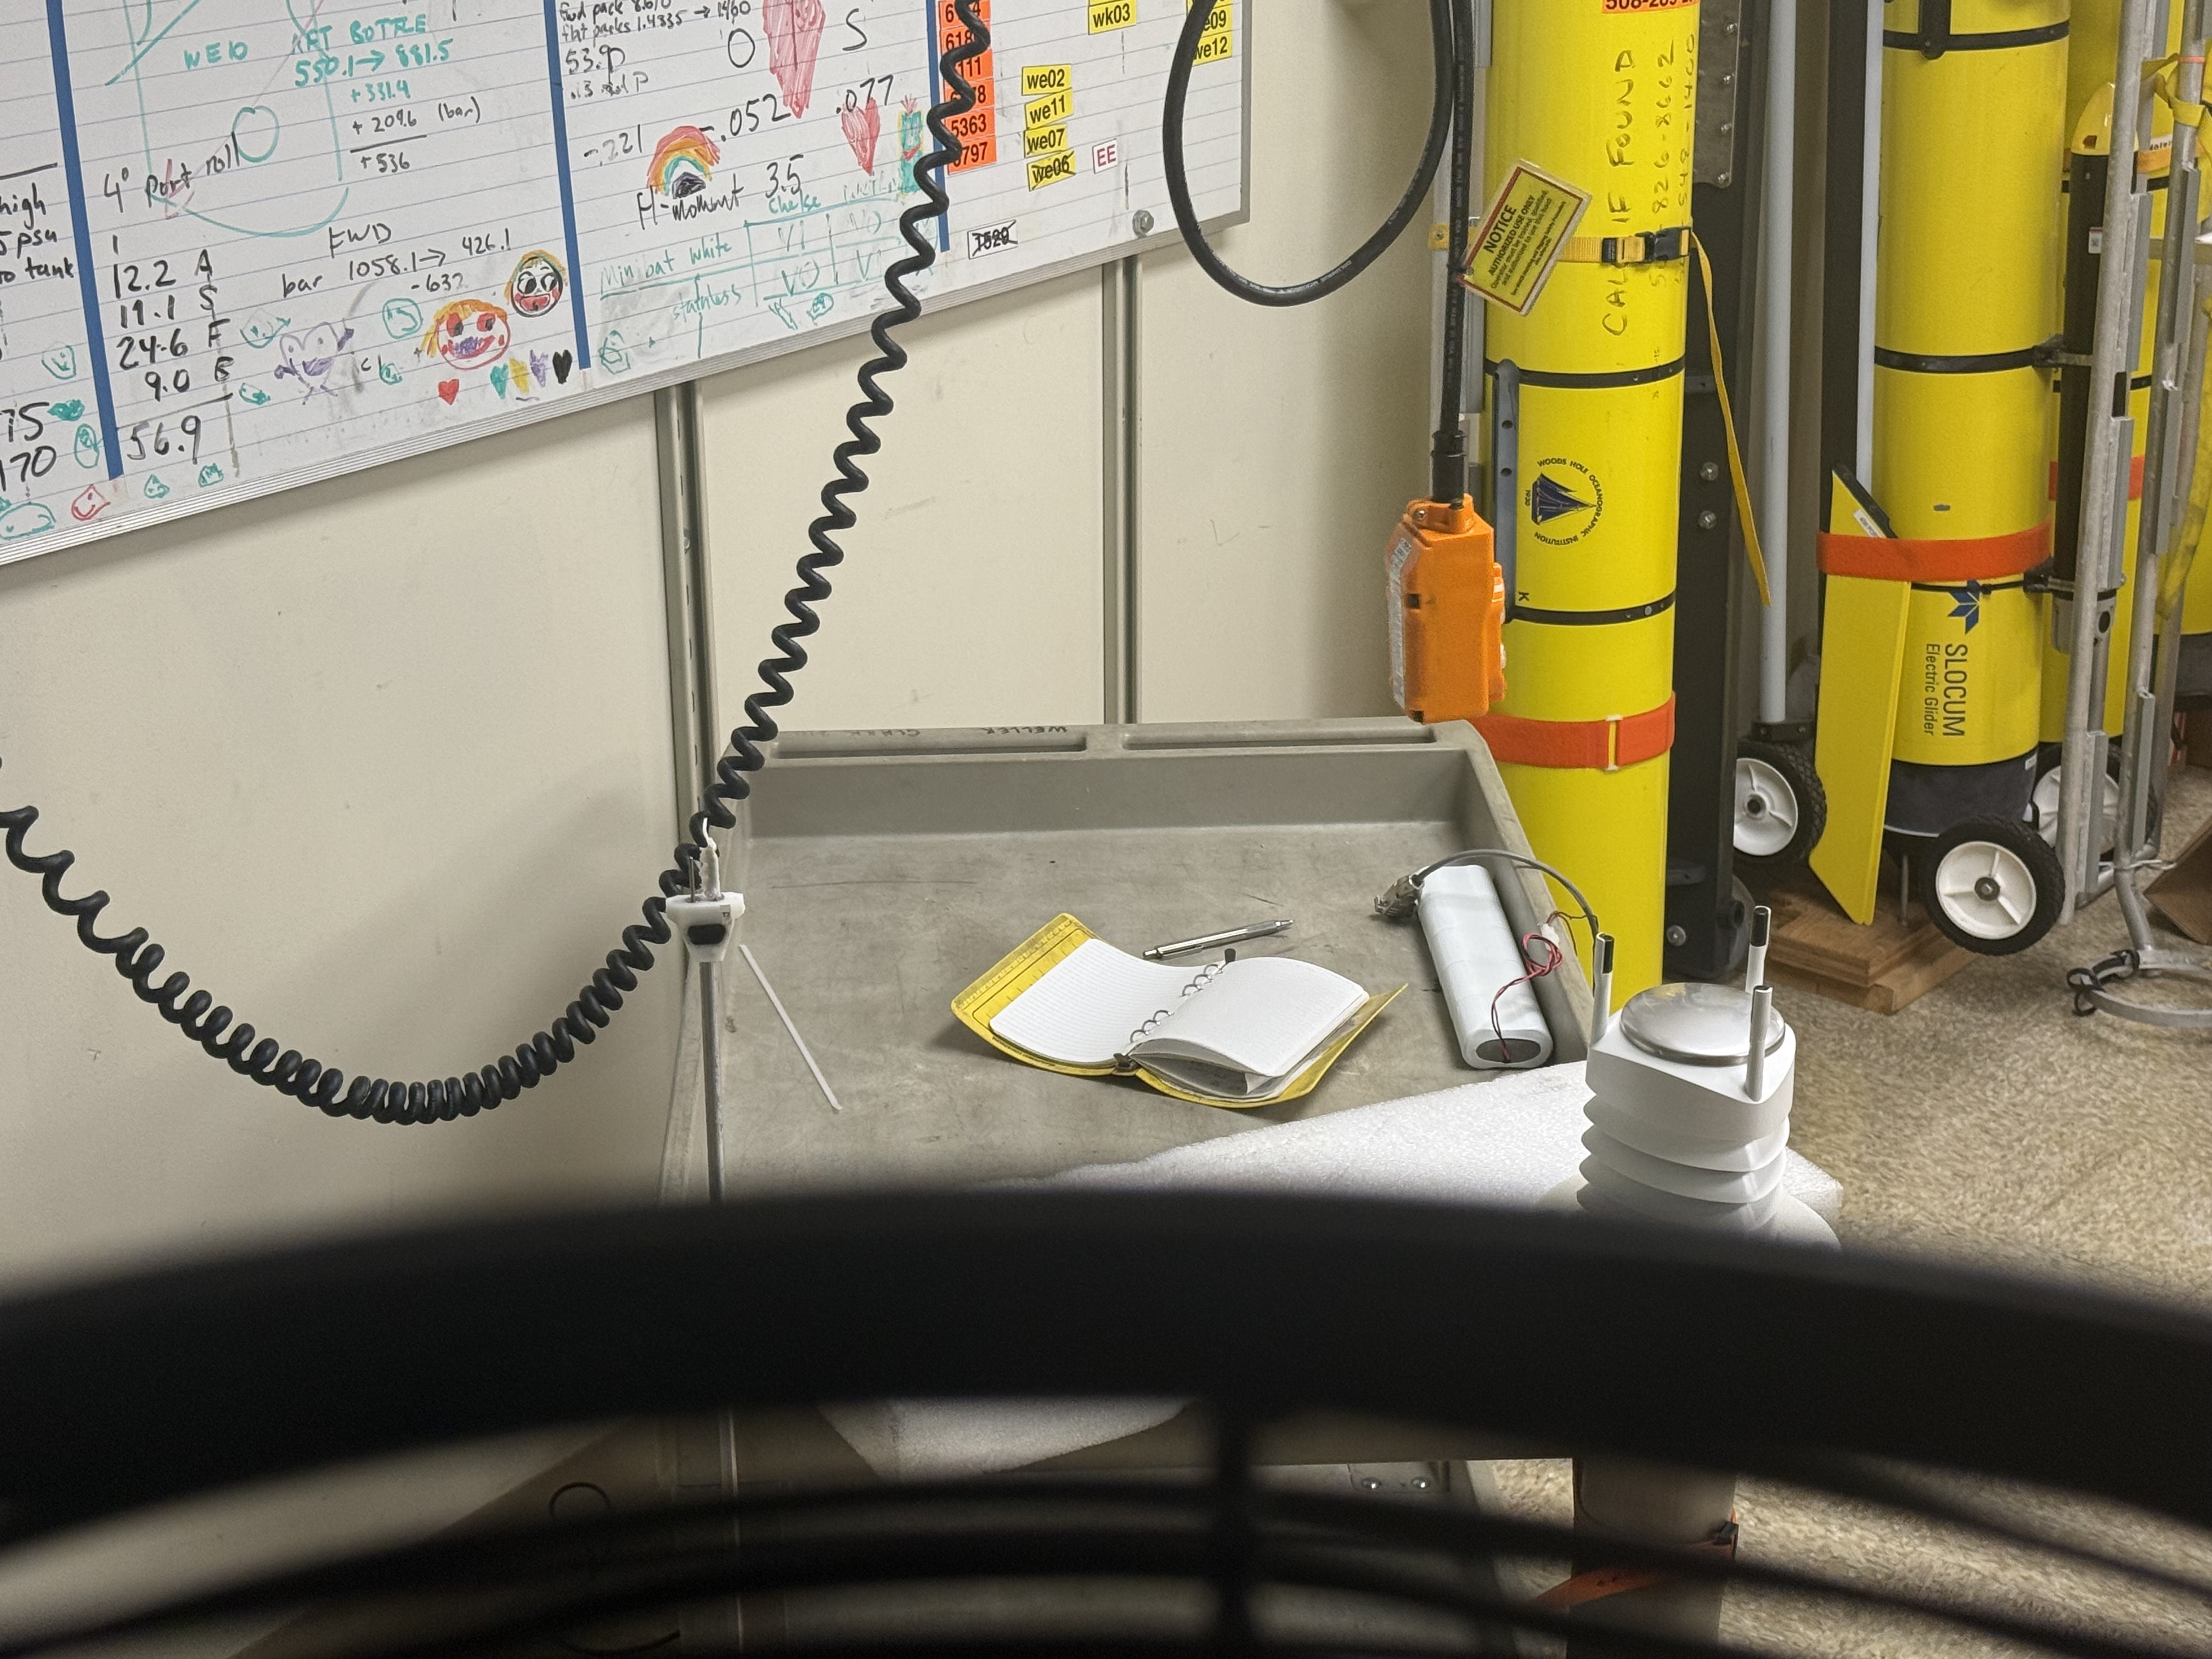
\includegraphics[width=0.48\linewidth,height=0.24\textheight,keepaspectratio]{../../data/20260629Lab/IMG_7610.jpeg}\\[0.8em]
  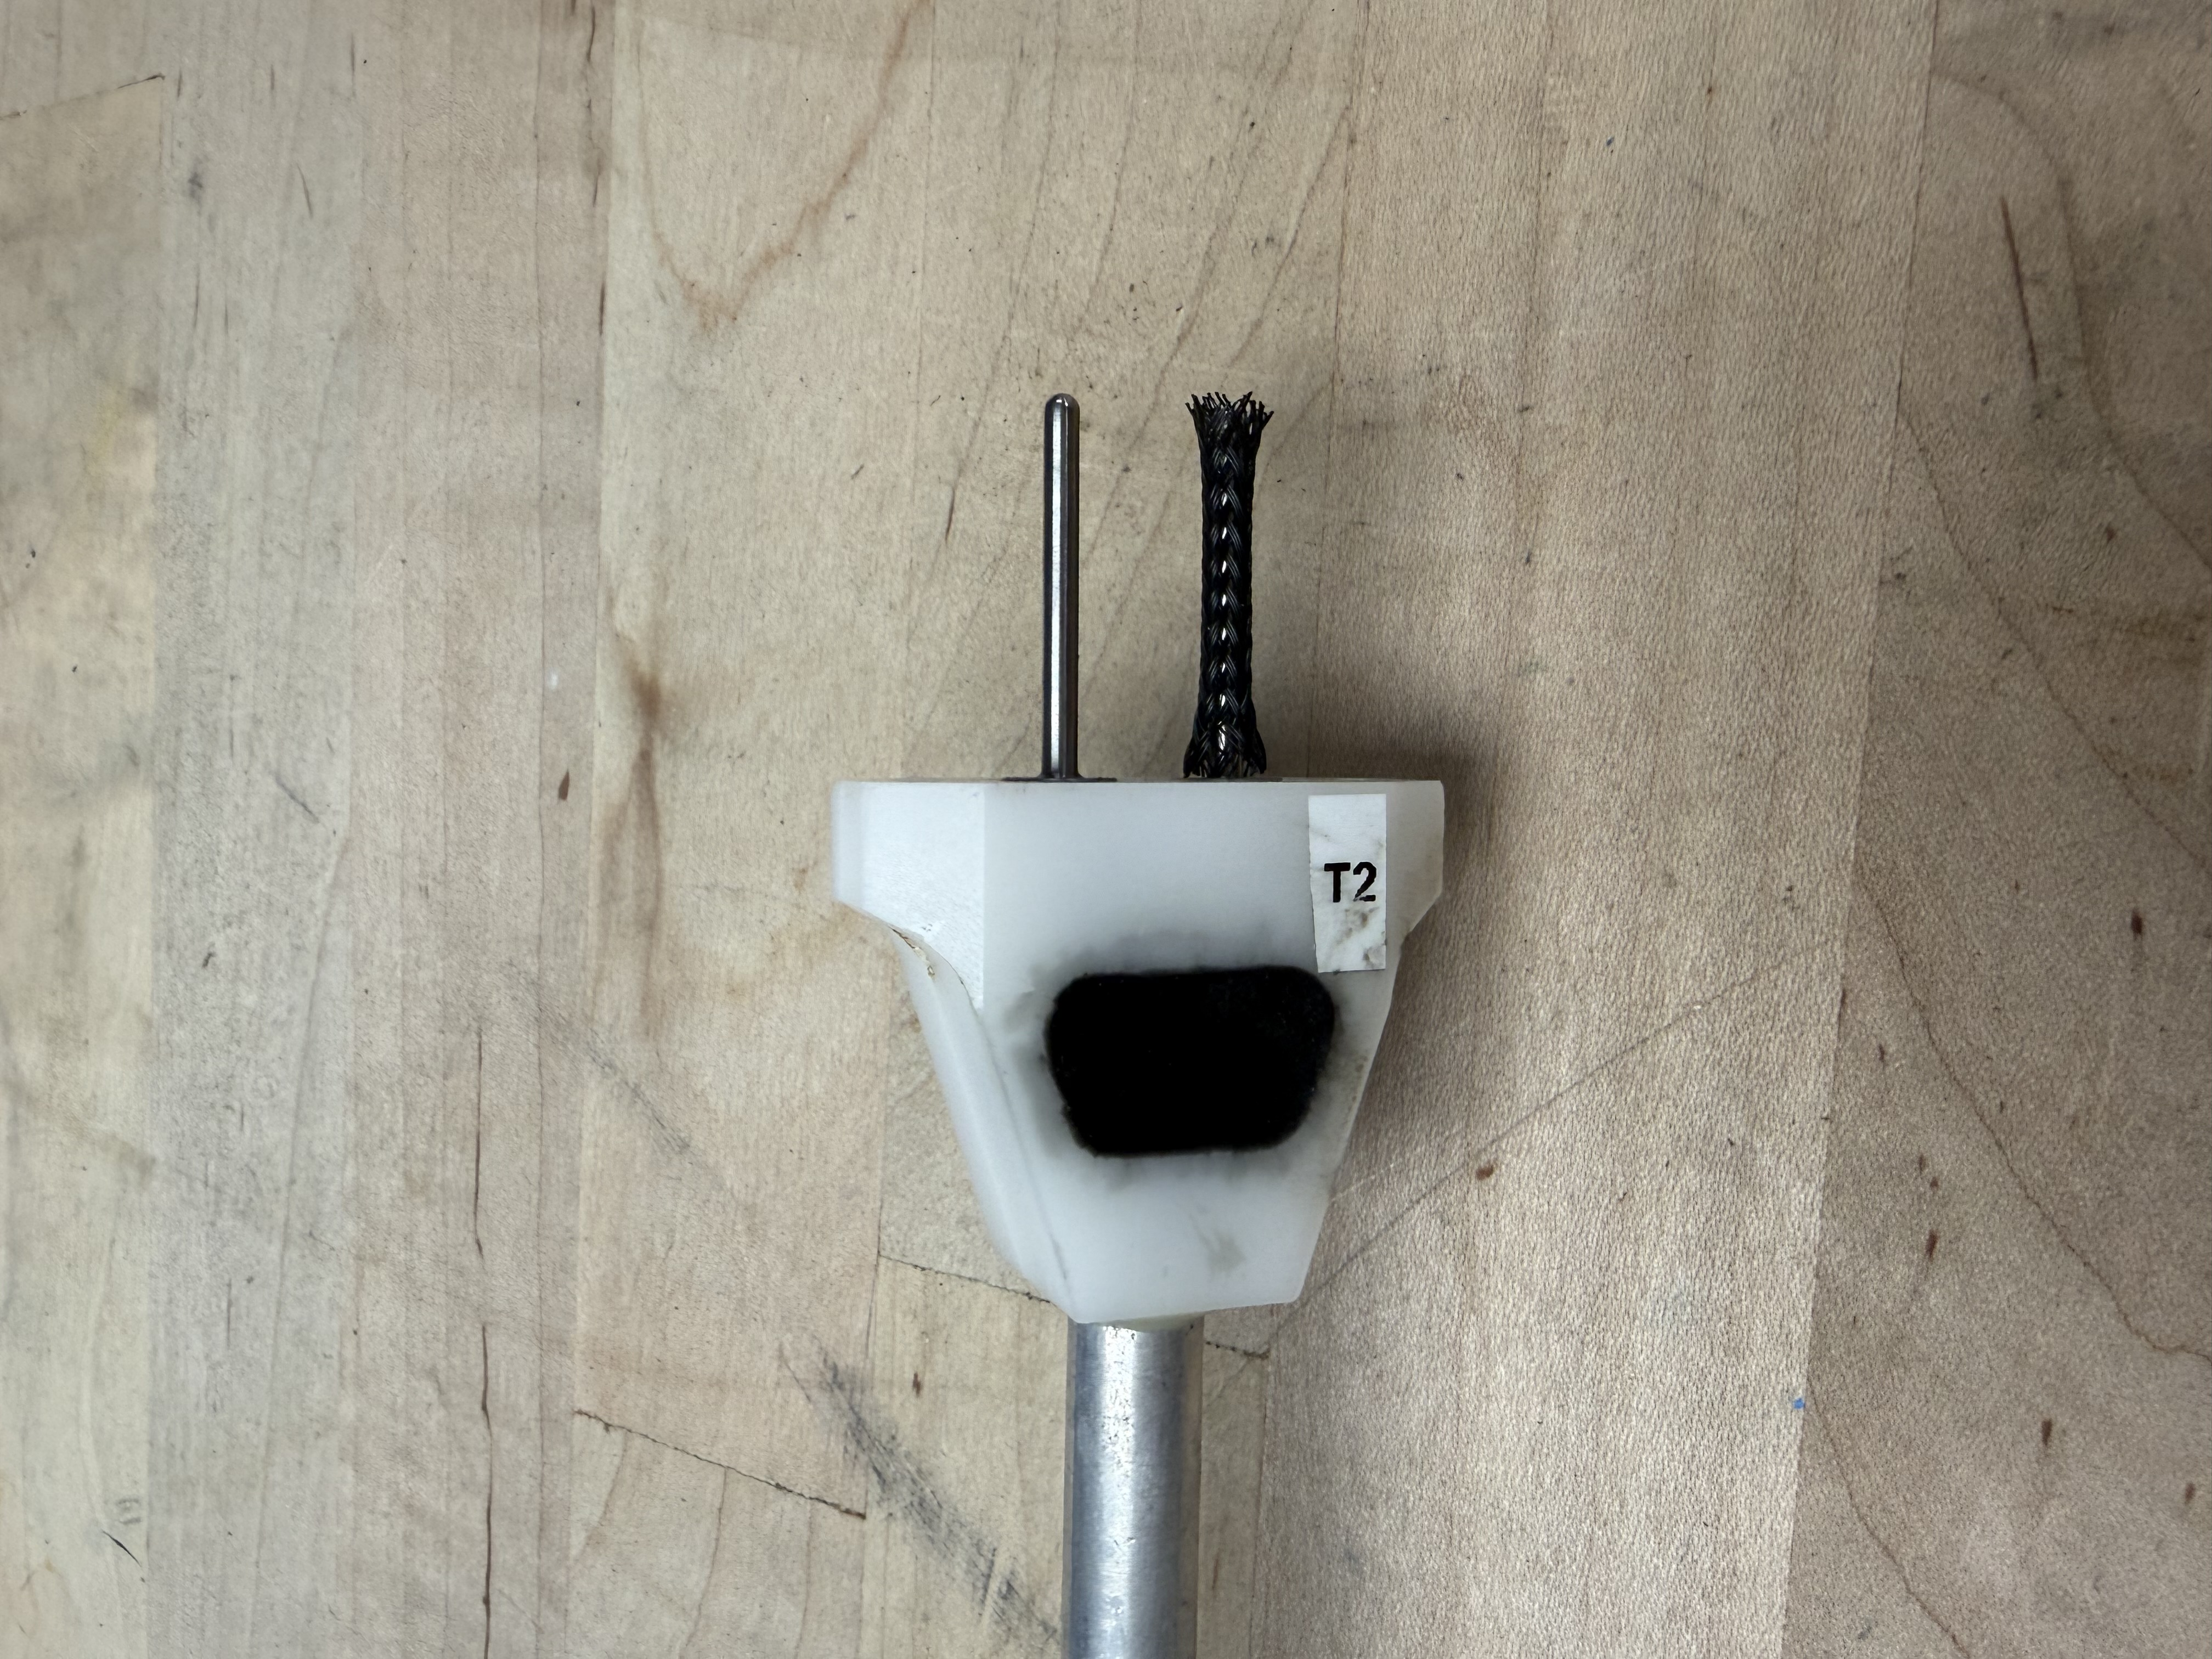
\includegraphics[width=0.31\linewidth,height=0.24\textheight,keepaspectratio]{../../data/20260629Lab/IMG_7611.jpeg}\hfill
  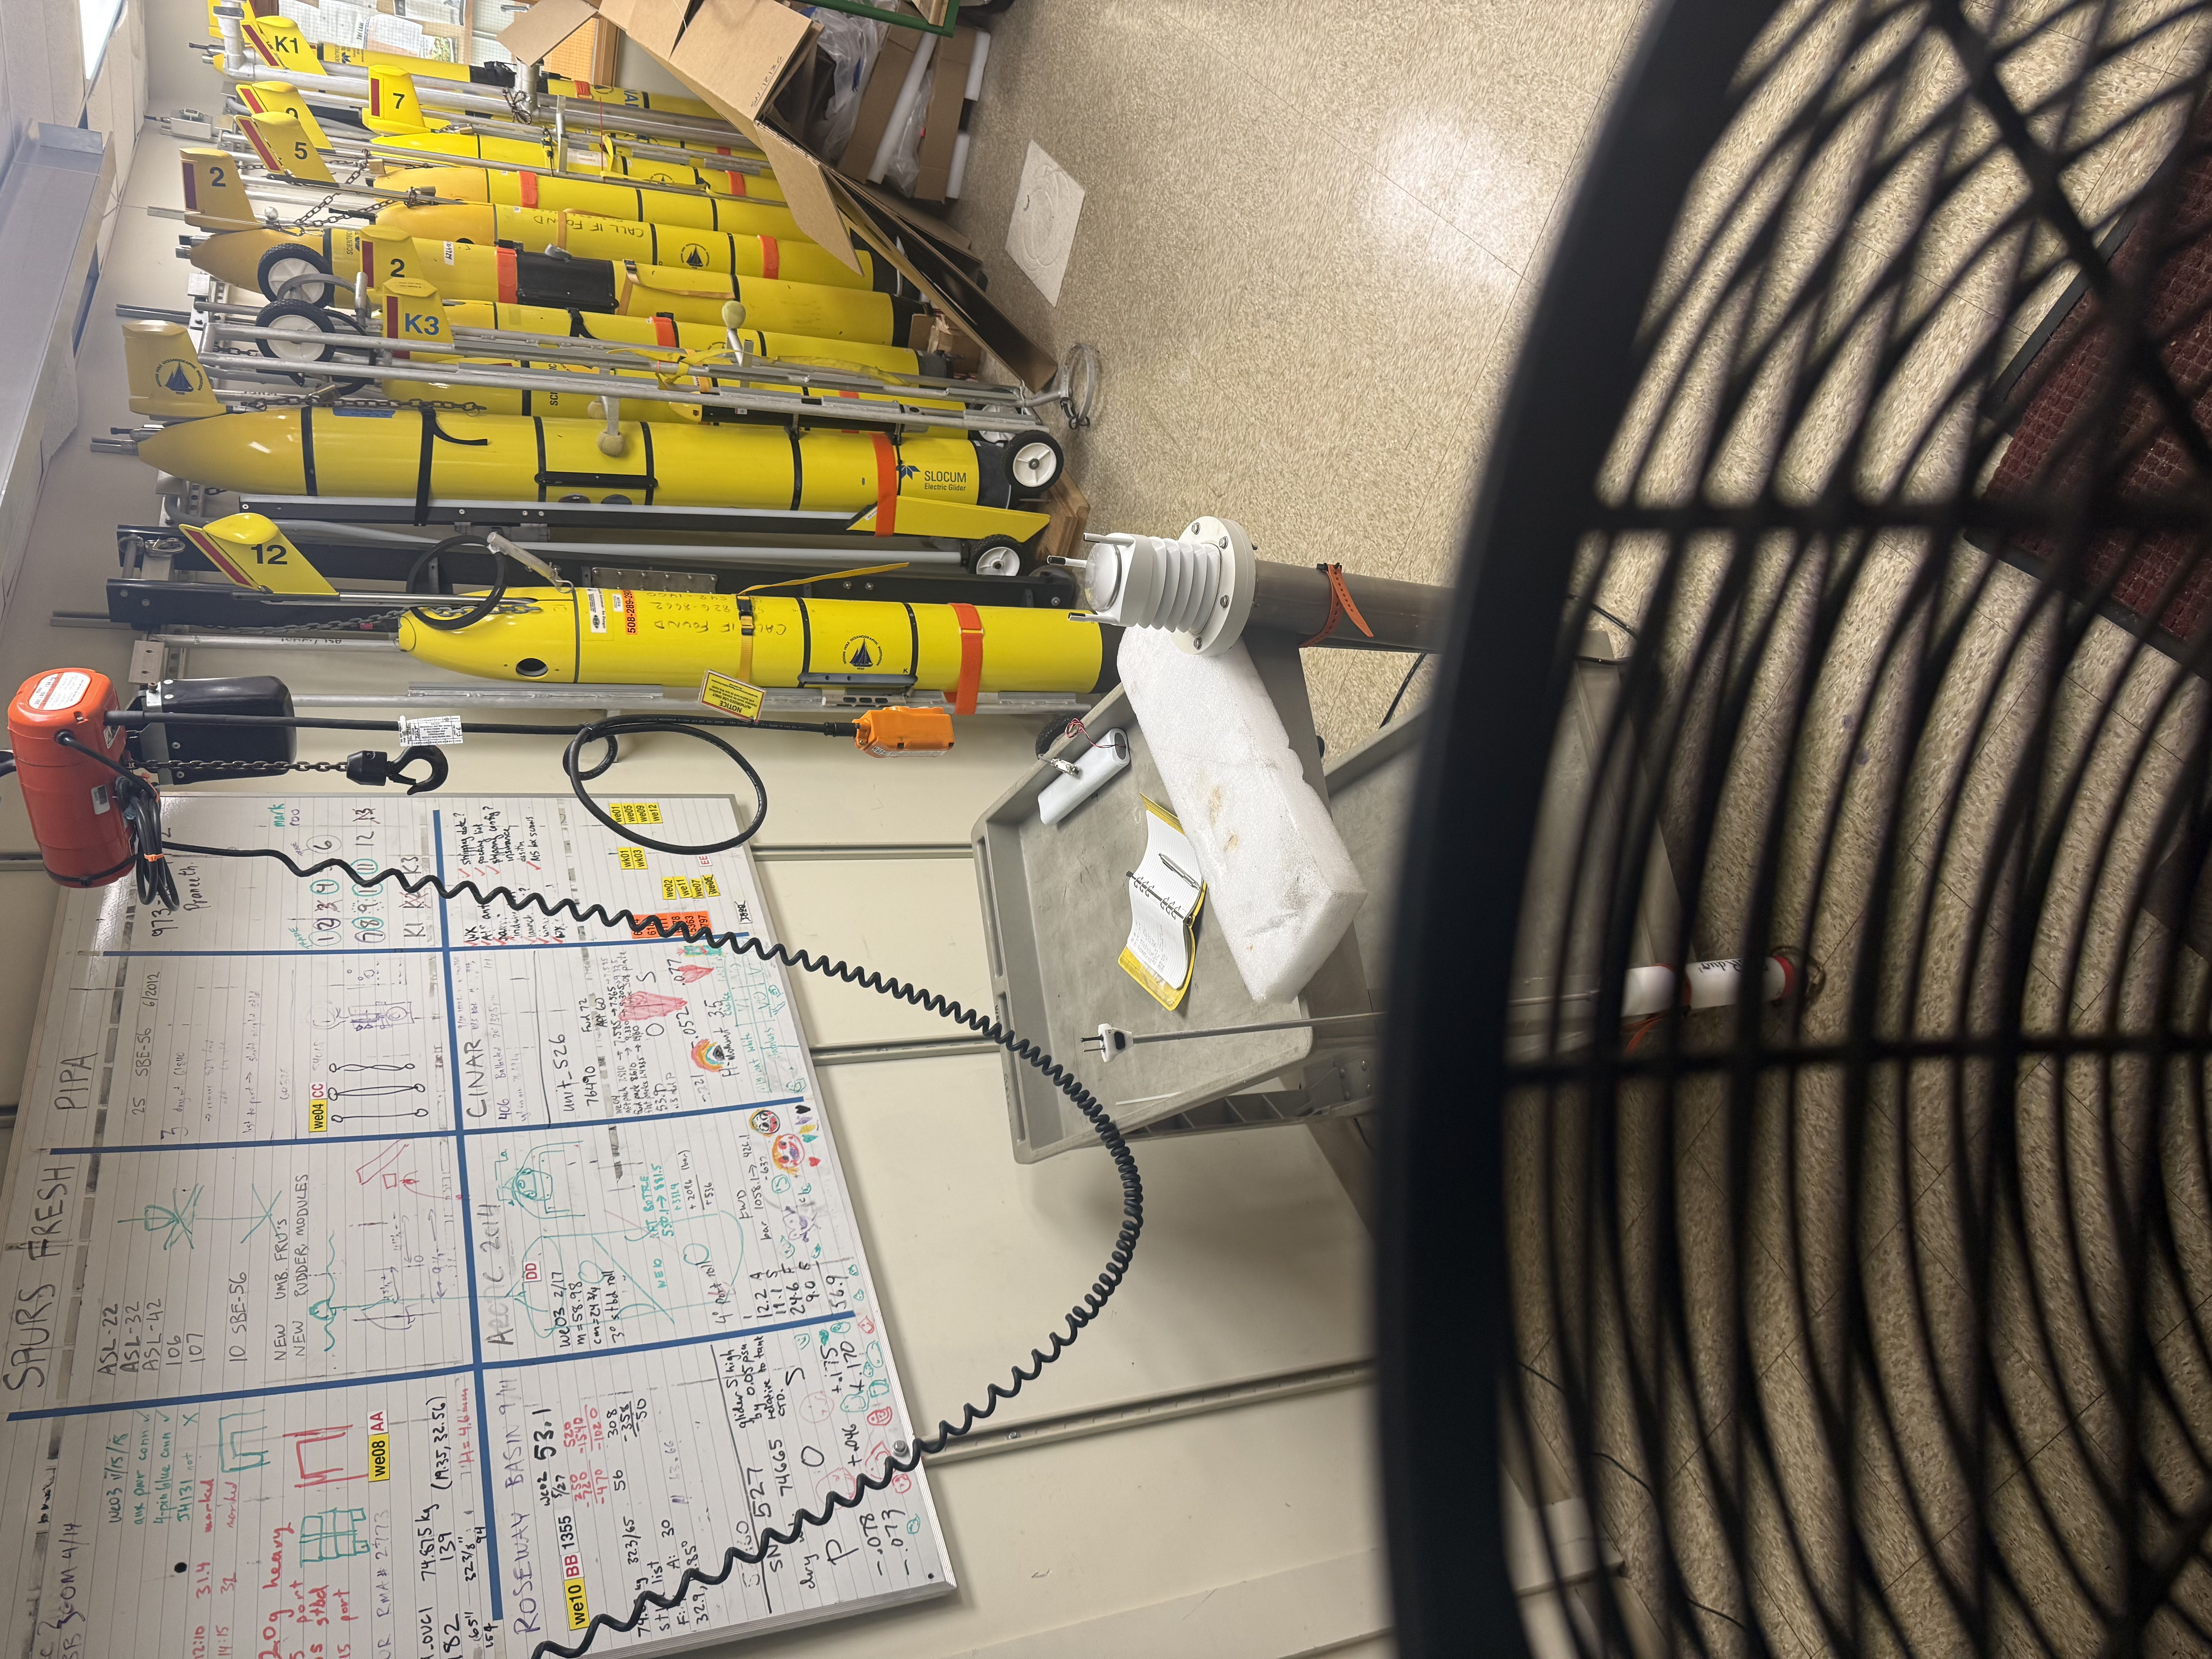
\includegraphics[width=0.31\linewidth,height=0.24\textheight,keepaspectratio]{../../data/20260629Lab/IMG_7612.jpeg}\hfill
  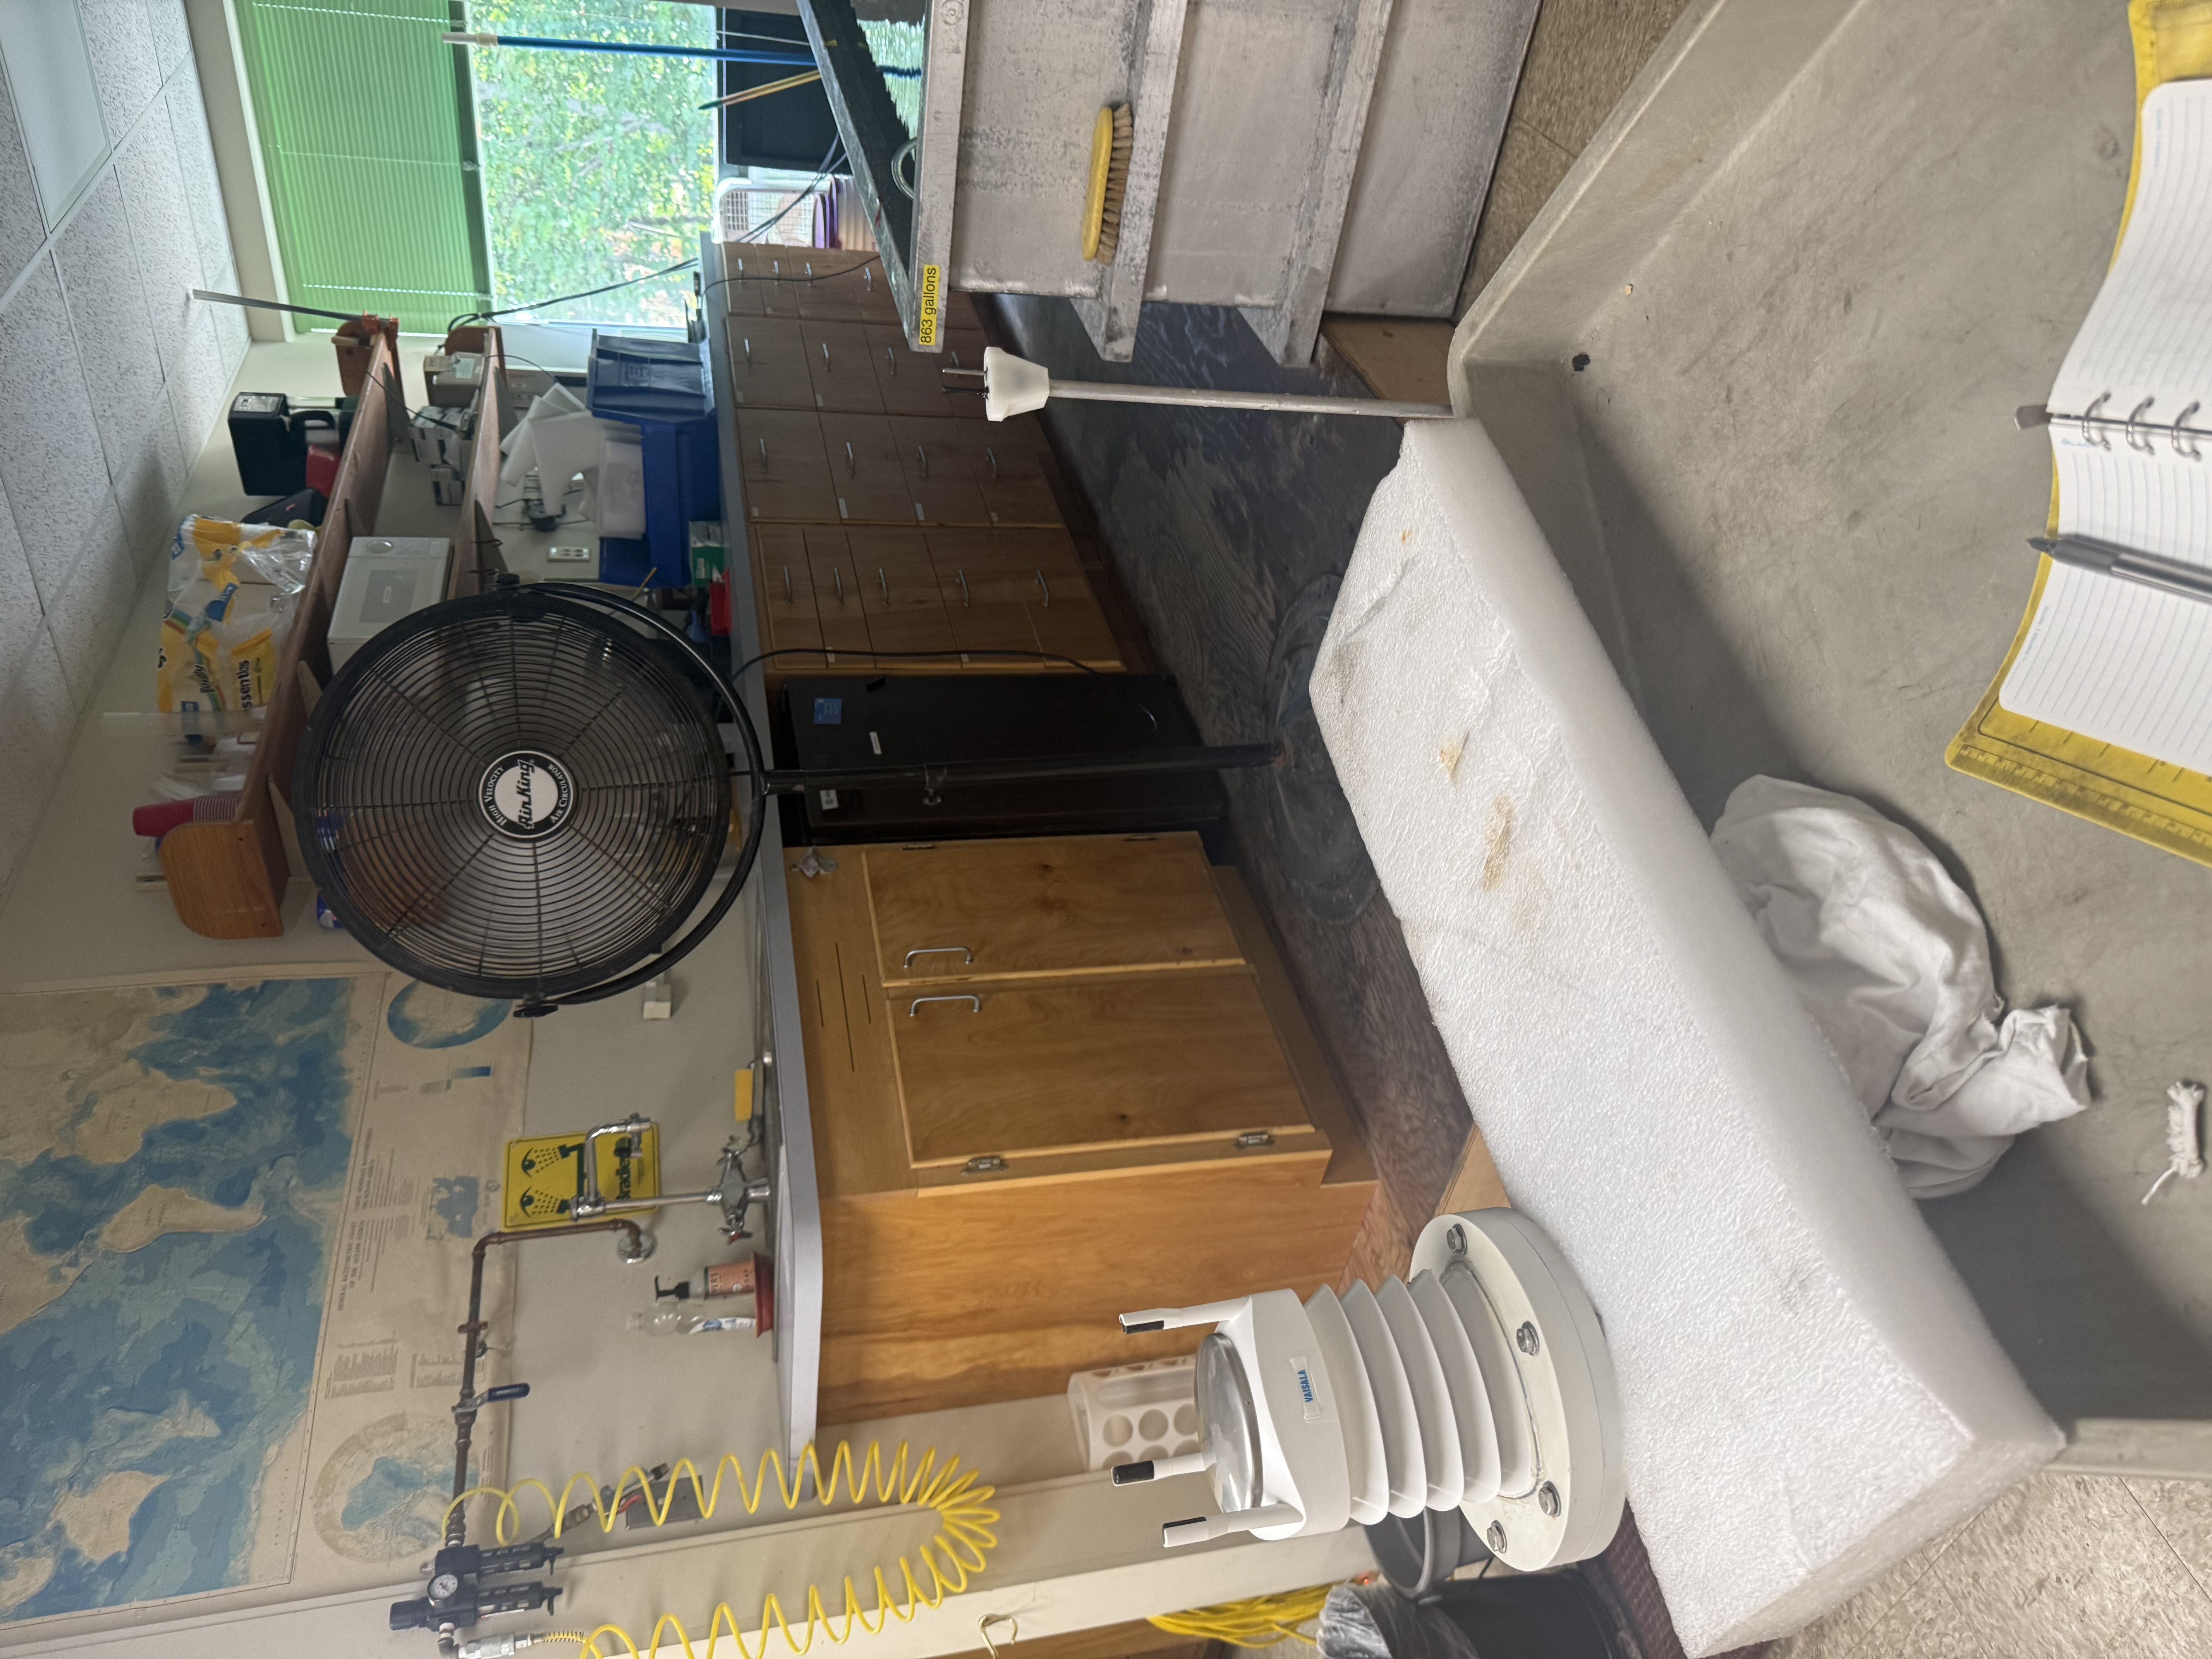
\includegraphics[width=0.31\linewidth,height=0.24\textheight,keepaspectratio]{../../data/20260629Lab/IMG_7613.jpeg}
  \caption{Setup photographs from \texttt{data/20260629Lab}. Top: June 29
  original-wick layout with the WXT520, SHS wet/dry-bulb mast, fan, and ballast
  tank. Bottom: June 30 plastic-wick follow-up, including the friction-fit wick
  close-up and wider fan-facing instrument layout.}
  \label{fig:photo_log}
\end{figure}

\section{Humidity: WXT520 vs.\ Psychrometric}

\begin{figure}[htbp]
  \centering
  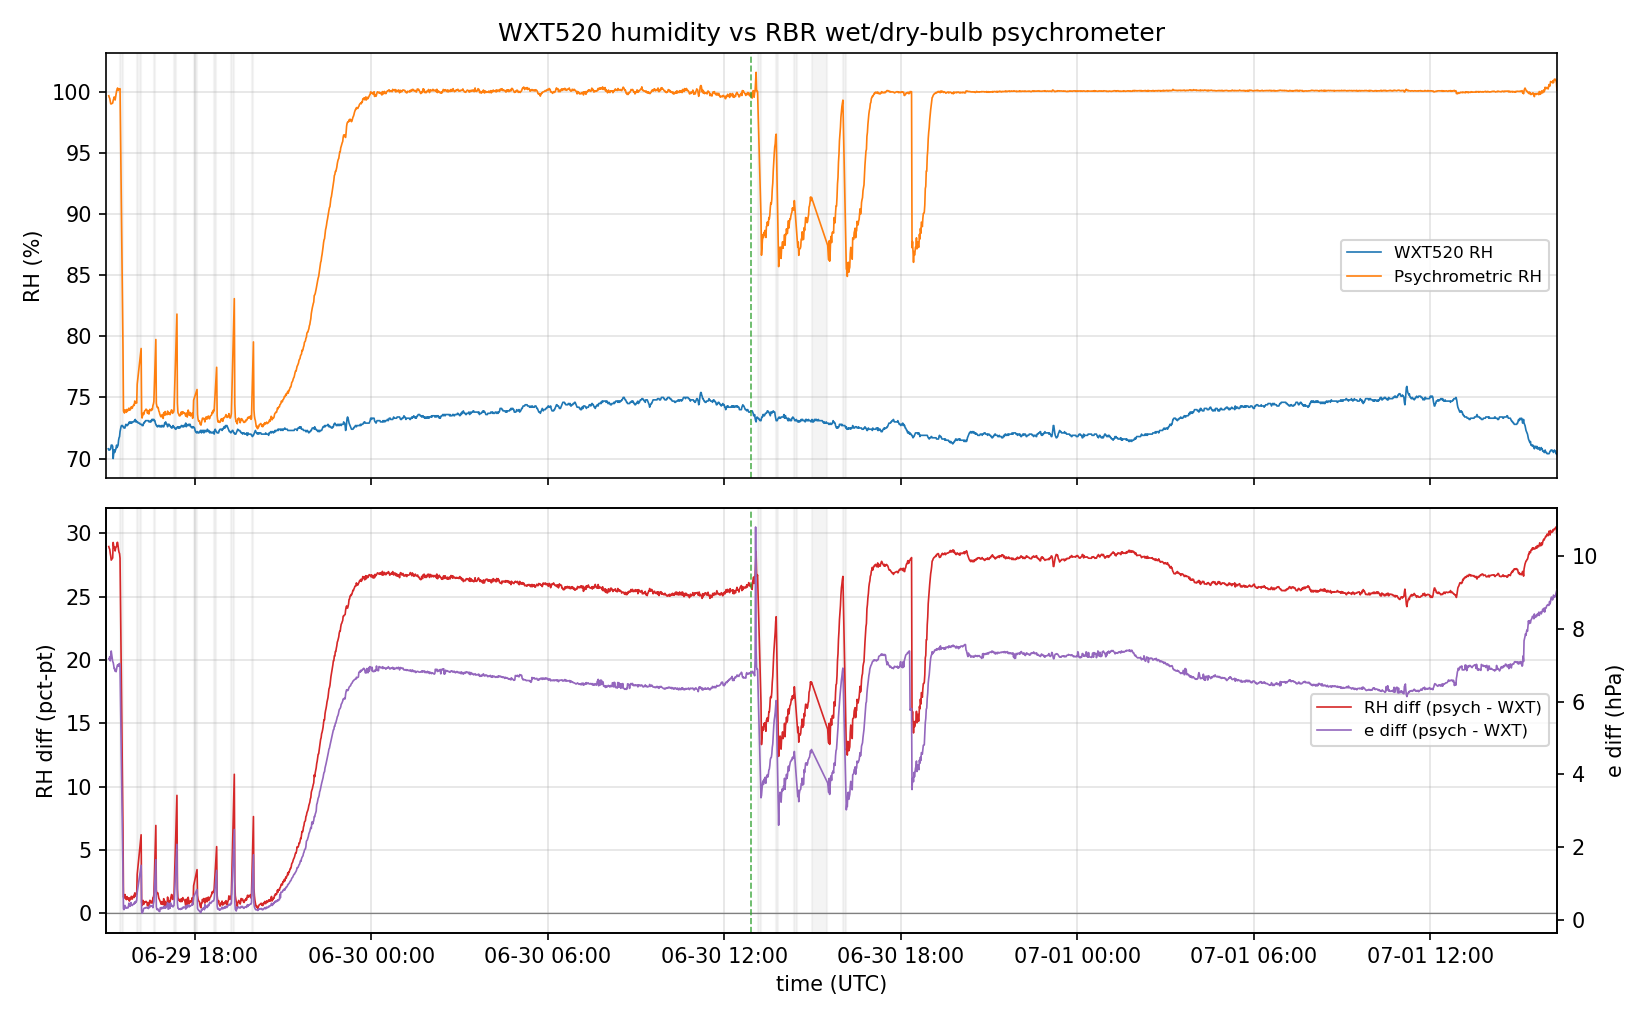
\includegraphics[width=\linewidth]{../../img/Lab20260629/Lab20260629_WXT_vs_psychrometric_humidity_report.png}
  \caption{Top: WXT520 RH and RBR wet/dry-bulb psychrometric RH. Bottom:
  psychrometric minus WXT RH difference and vapor-pressure difference. Grey
  bands mark in-water periods; the green dashed line marks the June 30
  plastic-wick change.}
  \label{fig:humidity}
\end{figure}

\begin{center}
\begin{tabular}{lrrrrr}
\toprule
Phase & N & WXT RH & psych RH & $\Delta$RH & $\Delta e$ \\
\midrule
2026-06-29 original wick & 263 & 72.47 & 74.23 & +1.75 & +0.52 \\
2026-06-30 plastic wick & 273 & 72.90 & 93.57 & +20.67 & +5.34 \\
\bottomrule
\end{tabular}
\end{center}

The original-wick day tracks the WXT520 closely during active in-air windows.
The plastic-wick day shows a much larger psychrometric humidity offset, so that
configuration should be treated as unresolved until the wick geometry and wetting
state are checked. The full post-test record remains useful for seeing wick
drying and long-term drift, but the table above uses only active in-air samples
from the note-defined test windows.

\section{Temperature and Tank Reference}

\begin{figure}[htbp]
  \centering
  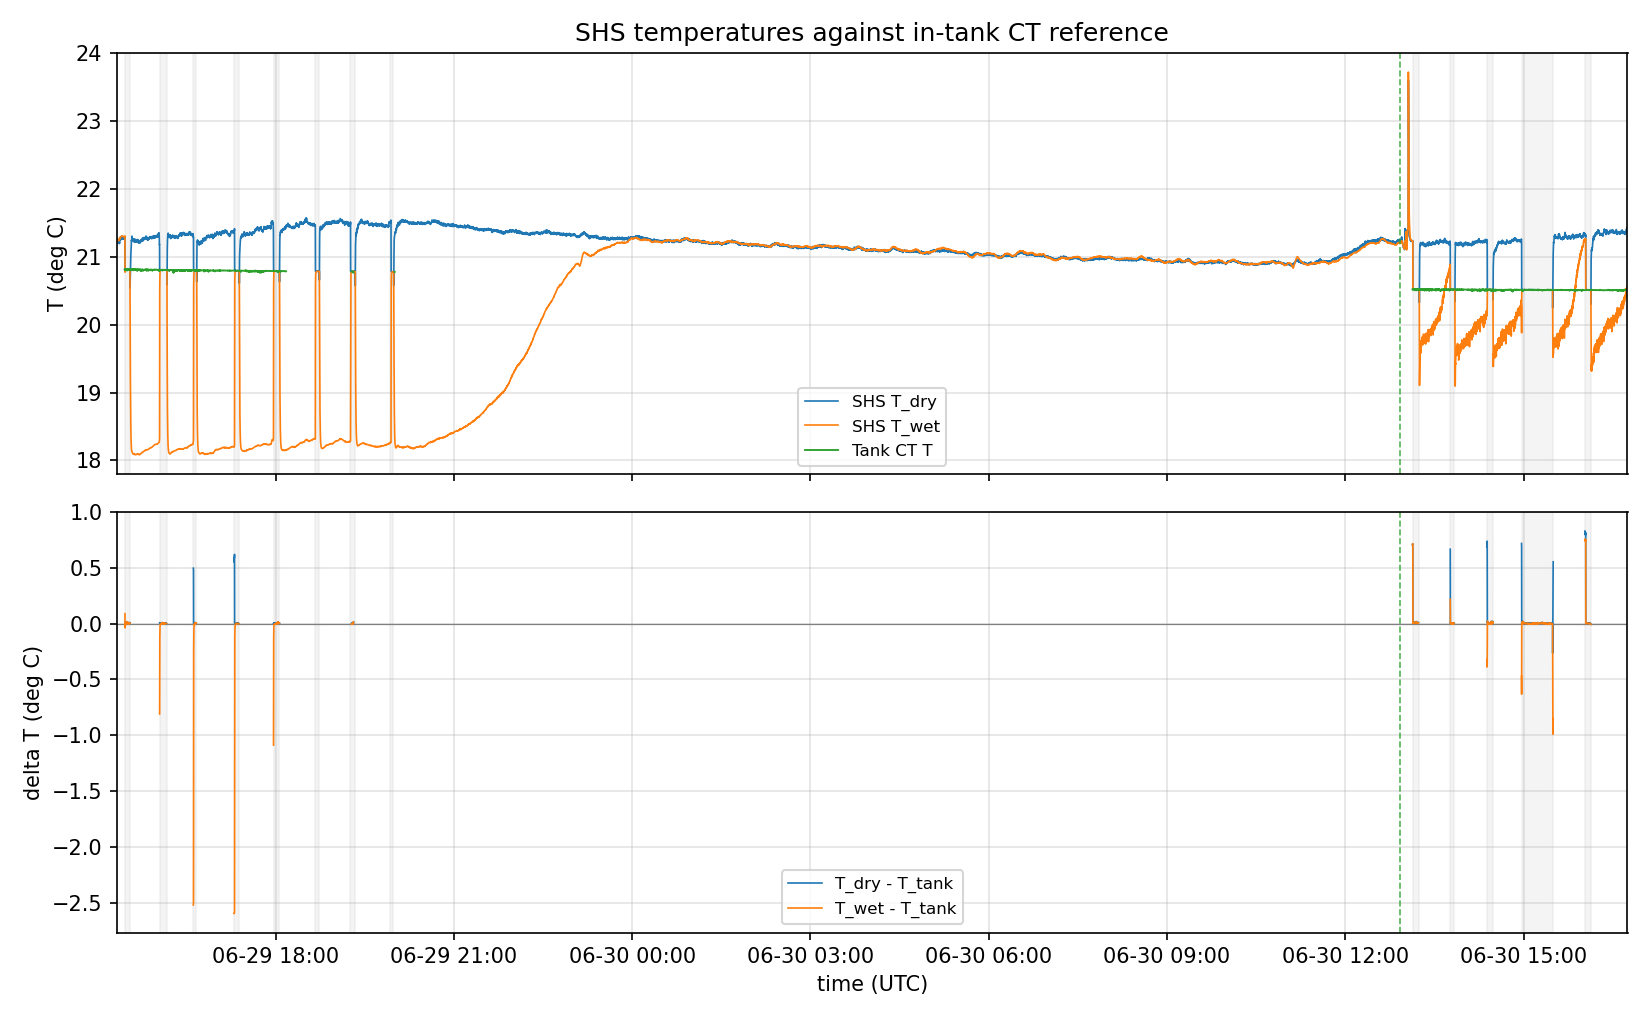
\includegraphics[width=\linewidth]{../../img/Lab20260629/Lab20260629_SHS_vs_tank_report.png}
  \caption{Top: SHS dry- and wet-bulb temperatures with the in-tank CT
  reference. Bottom: SHS minus tank-temperature residuals during periods with CT
  coverage. Grey bands mark in-water periods; the green dashed line marks the
  June 30 plastic-wick change.}
  \label{fig:tank}
\end{figure}

\begin{center}
\begin{tabular}{llrrrr}
\toprule
Cycle & Phase & $T_\text{tank}$ & $T_d-T_\text{tank}$ & $T_w-T_\text{tank}$ & N \\
\midrule
J29-IN-1 & 29 original wick & 20.810 & +0.006 & +0.001 & 101 \\
J29-IN-2 & 29 original wick & 20.805 & +0.003 & -0.014 & 141 \\
J29-IN-3 & 29 original wick & 20.799 & +0.043 & -0.273 & 61 \\
J29-IN-4 & 29 original wick & 20.794 & +0.077 & -0.375 & 101 \\
J29-IN-5 & 29 original wick & 20.788 & +0.003 & -0.018 & 121 \\
J29-IN-7 & 29 original wick & 20.783 & +0.113 & -0.437 & 101 \\
J30-IN-1 & 30 plastic wick & 20.517 & +0.041 & +0.040 & 121 \\
J30-IN-2 & 30 plastic wick & 20.517 & +0.018 & +0.006 & 81 \\
J30-IN-3 & 30 plastic wick & 20.513 & +0.053 & -0.024 & 121 \\
J30-IN-4 & 30 plastic wick & 20.511 & +0.009 & -0.017 & 641 \\
J30-IN-5 & 30 plastic wick & 20.511 & +0.115 & +0.105 & 121 \\
\bottomrule
\end{tabular}
\end{center}

\section{Response Times}

\begin{figure}[htbp]
  \centering
  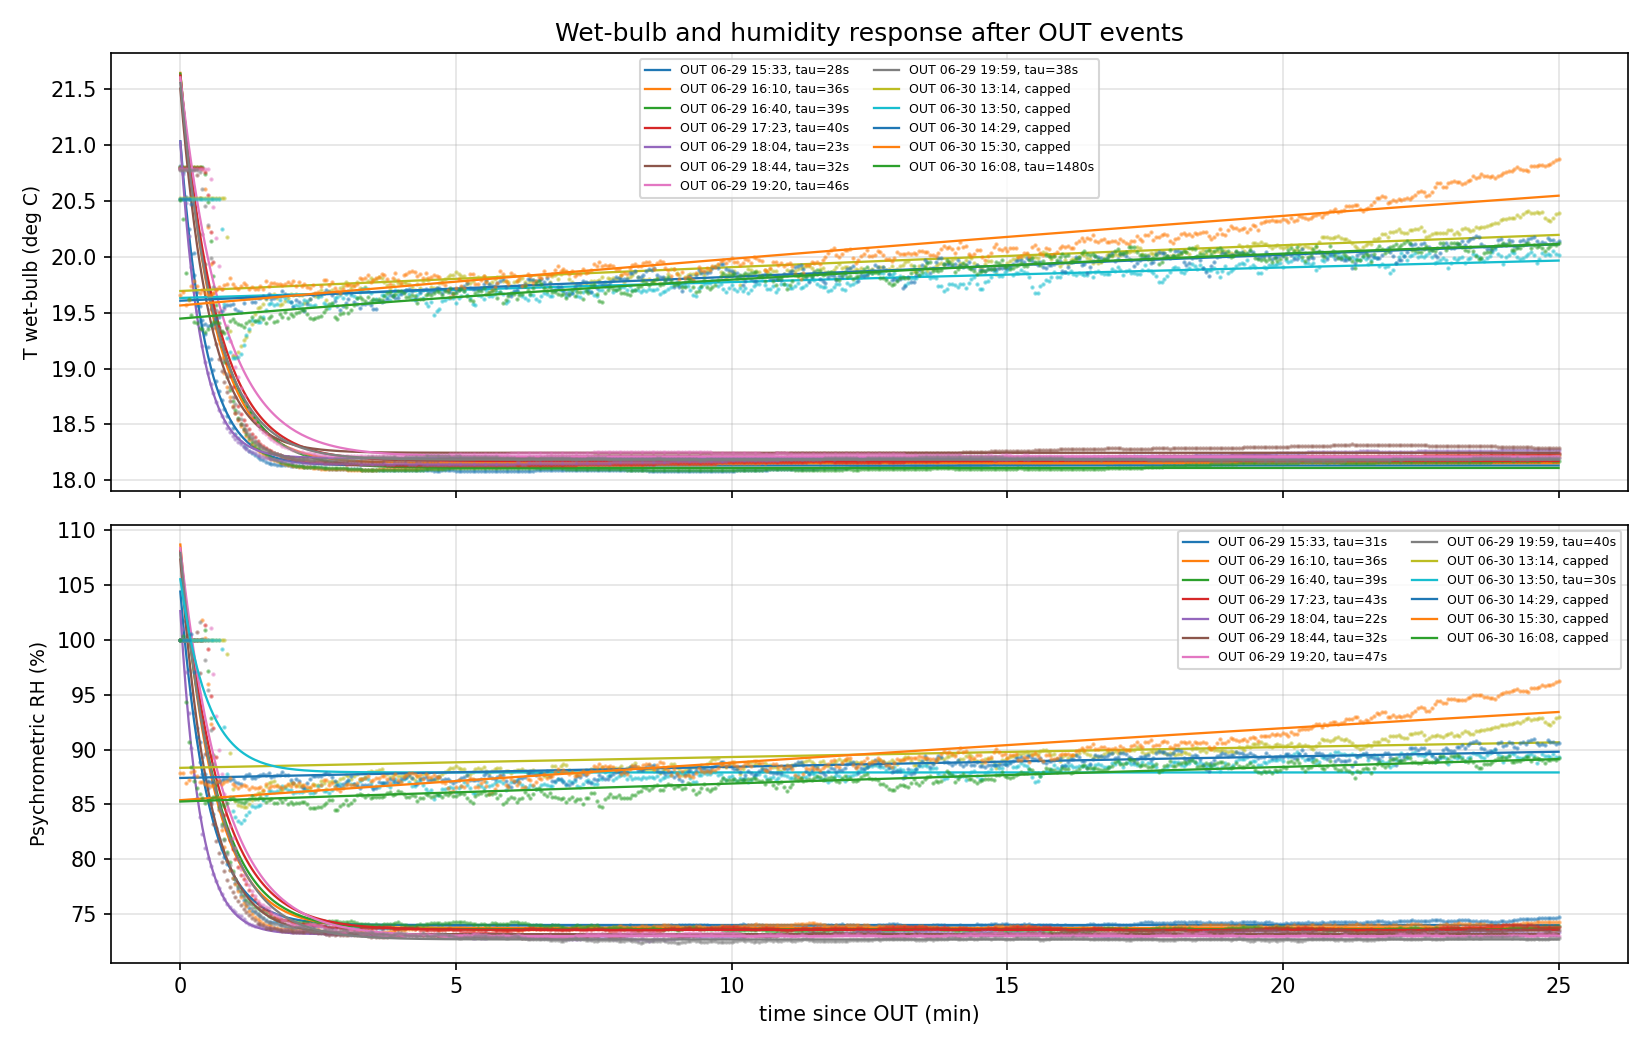
\includegraphics[width=\linewidth]{../../img/Lab20260629/Lab20260629_response_time_report.png}
  \caption{Wet-bulb temperature and psychrometric-RH trajectories aligned to
  each OUT event. Dots are observations and lines are exponential fits; labels
  list the OUT time and fitted time constant, or ``capped'' when the fit reached
  the upper bound. Fit windows run from OUT to
  $\min(\text{OUT}+25\,\text{min},\,\text{next IN})$.}
  \label{fig:response}
\end{figure}

\begin{center}
\begin{tabular}{lrrrrr}
\toprule
Phase & N & $\tau_{T_d}$ & $\tau_{T_w}$ & $\tau_\text{dep}$ & $\tau_\text{RH}$ \\
\midrule
2026-06-29 original wick & 8 & 47 & 37 & 38 & 38 \\
2026-06-30 plastic wick & 5 & 56 & $\geq7200^*$ & $\geq7200^*$ & $\geq7200^*$ \\
\bottomrule
\end{tabular}

\smallskip{\footnotesize $^*$ Fit reached the 7200 s upper bound; treat those
values as non-exponential or unresolved rather than physical time constants.}
\end{center}

\begin{center}
\begin{tabular}{lrrrr}
\toprule
Phase & N & median $t_\text{knee}$ (s) & median $t_{63}$ (s) & RH at plateau (\%) \\
\midrule
2026-06-29 original wick & 8 & 90 & 48 & 73.5 \\
2026-06-30 plastic wick & 5 & 66 & 30 & 88.5 \\
\bottomrule
\end{tabular}
\end{center}

\section{Diagnostics}

The full multi-panel diagnostics are still generated for traceability, but are
omitted here to keep the report focused. They remain in
\texttt{img/Lab20260629} and \texttt{data/20260629Lab} alongside the
streamlined report figures.

\section{Generated Files}

\begin{itemize}
  \item \texttt{data/20260629Lab/RBR\_SHS/psychrometrics\_20260629.csv}
  \item \texttt{data/20260629Lab/compare\_SHS\_tank\_20260629.csv}
  \item \texttt{data/20260629Lab/compare\_WXT\_psychrometric\_20260629.csv}
  \item \texttt{data/20260629Lab/response\_time\_20260629.csv}
  \item \texttt{data/20260629Lab/wet\_bulb\_settling\_20260629.csv}
\end{itemize}

\end{document}
